\chapter{Sustainable development}

At a time when France is concerned about the ecological impact on the planet of air conditioners to cool our rooms during hot weather, this problem does not seem to be at the heart of UTP's concerns.

As outdoor temperatures are very high in Malaysia, all buildings (train station, restaurants, hotels, etc.) and cars are equipped with air conditioners. However, the settings of these are often far too cold ($\approx 20^{\circ}C$) and force us to wear warm and long clothes inside the buildings despite the outside temperature greatly exceeding $30^{\circ}C$ throughout our stay.

\begin{figure}[h]
  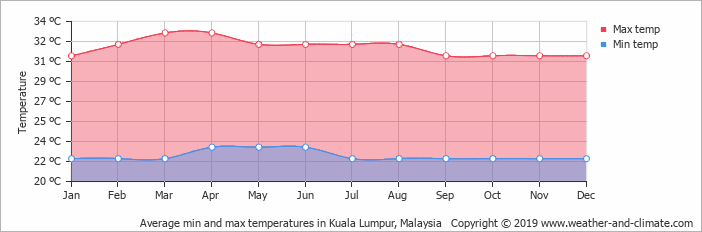
\includegraphics[width=1\linewidth]{content/imgs/temp.png}
  \caption{Minimum and maximum average temperatures in Malaysia, in the capital city}
  \label{fig:climate}
\end{figure}

Despite the excessive use of air conditioners, the university's recent buildings do not have thermal insulation comparable to recent buildings built in France. To take just one example, I worked in the university library, which has a huge glass facade lined with doors, also glazed, allowing the freshness of the buildings to be felt for several metres outside. In addition, the air conditioners in the university's laboratory rooms remain on most of the time all day long despite the absence of people in the air-conditioned rooms, and with the doors open (which open directly to the outside).

According to the university website \cite{utp_gender}, special attention is being paid to promoting gender diversity within the university, whether at the level of students, employees and teaching staff.
